%
% chapter.tex -- Beschreibung des Inhaltes
%
% (c) 2025 Prof Dr Andreas Müller
%
% !TeX spellcheck = de_CH
\chapter{Einleitung
\label{chapter:einleitung}}
\kopflinks{Einleitung}

Die Entwicklung der Infinitesimalrechnung durch Newton und Leibniz
gehört zu den grössten Schritten, die die Mathematik in ihrerer
mehrtausendjährigen Geschichte genommen hat.
Dazu waren mehrere neue Begriffe nötig, die sich im Laufe der
Entwicklung der Analysis herauskristallisierten und über die
Jahre immer klarer definiert wuden.
Der Funktionsbegriff formalisiert die Idee der Abhängigkeit einer
Grössen von einer oder mehreren anderen Grössen.
\index{Funktionsbegriff}%
Die Ableitung idealisiert die Änderung einer abhängigen Grösse
\index{Ableitung}%
unter kleinen Änderungen der unabhängigen Variable für den Fall
``unendlich kleiner'' Änderungen.
Das Integral rekonstruiert den Verlauf einer Funktion aus ihren
\index{Integral}%
infinitesimalen Änderungen.

Der Erfolg der Infinitesimalrechnung basiert aber nicht nur auf
den genannten Abstraktionsleistungen, sondern vor allem auch auf
dem algebraischen Kalkül, der zu Ihrer Anwendung erfunden worden ist.
Durch die fast mechanische Anwendung einfacher Regeln können 
Ableitungen und Integrale berechnet werden, ohne dass der Anwender
sich über ``unendlich kleine'' Grössen oder unendlich Summe solcher 
Grössen Gedanken machen müsste.

Im 19.~Jahrhundert begannen sich jedoch Risse im Fundament der
Infinitesimalrechnung zu bilden.
Der sorglose Umgang mit unendlich kleinen Grössen ist nur zum
Preis von Widersprüchen zu haben.
Die moderne Definition von Konvergenz und Grenzwert stellen die
Analysis auf eine solide Basis.
\index{Konvergenz}%
\index{Grenzwert}%
Die algebraischen Eigenschaften bleiben dabei unangetastet.

Heute präsentiert sich die Analysis von zwei Seiten.
Einerseits ist sie ein technisch ausgefeiltes System von Definitionen
und Sätzen, welches Antworten zu Fragen liefert, die man etwas salop mit
unendlich kleinen oder unendlichen Grössen assoziieren kann.
Andererseits ist es sie ein leistungsfähiger algebraischer Werkzeugkasten,
mit dem Ableitungen und Integrale auf mechanisch Art berechnet werden
können.
In keinem Gebiet der Analysis werden diese zwei Seiten so deutlich
wie in der komplexen Analysis, die in den ersten Kapiteln dieses
Buches entwickelt wird.
Die Existenz einer Ableitung einer komplexen Funktion hat weitreichende
algebraische Folgen: Real- und Imaginärteil sind über die
Cauchy-Riemann-Differentialgleichungen miteinander verbunden und
\index{Cauchy-Riemann-Differentialgleichungen}%
die Funktionswerte und Ableitungen in einem Punkt legen die Funktion
für alle möglichen Argument fest.

Während man sich reell differenzierbare Funktionen als beliebig flexibel
vorstellen kann, scheinen komplexe differenzierbare Funktionen in dem
Sinne starr zu sein, dass sie durch algebraische Eigenschaften bestimmt
sind.
Es überrascht daher wenig, dass sich im Rahmen der komplexen Analysis 
nun auch eine Antwort auf die schwierigen Frage geben lässt, ob sich zu
einem als Term formulierten Integranden auch ein Funktionsterm für die
Stammfunktion finden lässt.
Dieses als ``Integration in geschlossener Form'' bekannte Problem wird
in den letzten zwei Kapiteln des ersten Teils behandelt.

%
% 1-frueh.tex
%
% (c) 2026 Prof Dr Andreas Müller
%
\section{Die frühe Entwicklung der Analysis
\label{buch:einleitung:section:frueh}}
\kopfrechts{Die frühe Entwicklung der Analysis}

\subsection{Frühe Vorläufer
\label{buch:einleitung:frueh:subsection:vorlaeufer}}
%
% fig-parabel.tex
%
% (c) 2026 Prof Dr Andreas Müller
%
\begin{figure}
\centering
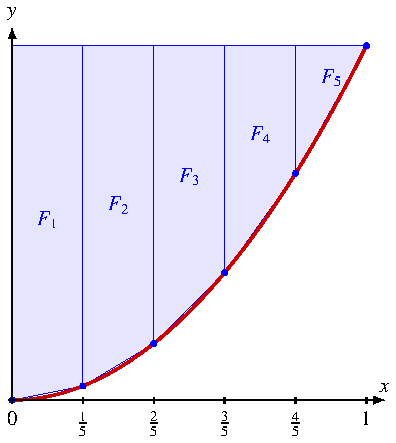
\includegraphics{chapters/000-einleitung/images/parabel.pdf}
\caption{Exhaustion der Parabel $y=x^2$
\label{buch:einleitung:fig:parabel}}
\end{figure}
%
Schon Archimedes war in der Lage, den Flächeninhalt eines
Parabelbogens zu bestimmen.
\index{Archimedes}%
\index{Parabelbogen}%
Mit seiner Methode der Exhaustion approximierte er durch Polygone,
\index{Exhaustion}%
deren Flächeninhalt mit rein algebraischen Methoden bestimmt werden
konnte.
Durch feiner werdende Unterteilung der Polygone konnte eine beliebig
genaue Näherung gefunden werden.
Den Parabelbogen $y=x^2$ mit $x\in [0,1]$ (siehe
Abbildung~\ref{buch:einleitung:fig:parabel}) kann man z.~B.~durch Unterteilung
in $n$ Stützstellen $x_i = \frac{i}{n}$, $i=0,\dots,n$, als Vereinigung
von Trapezen mit jeweils dem Flächeninhalt
\begin{align*}
|F_i|
&=
\frac12 \biggl(
\biggl( 1-\frac{(i-1)^2}{n^2} \biggr)
+
\biggl( 1-\frac{i^2}{n^2} \biggr)
\biggr)
\cdot
\frac{1}{n}
\\
&=
\frac1{2n^3}\bigl(
n^2-(i-1)^2+n^2-i^2
\bigr)
=
\frac1{2n^3}\bigl(
2n^2
-1+2i-2i^2
\bigr)
\end{align*}
betrachten.
Die Summe dieser Flächen ist
\begin{align}
F(n)
&=
\sum_{i=1}^n
F_i
=
\sum_{i=1}^n
\frac1{2n^3}
\bigl(
2n^2
-1+2i-2i^2
\bigr)
\notag
\\
&=
\frac1{2n^3}
\sum_{i=1}^n
\bigl(
2n^2
-1+2i-2i^2
\bigr)
=
1
-
\frac1{2n^3}
\biggl(
-
\sum_{i=1}^n 1
+
2
\sum_{i=1}^n i
-
2
\sum_{i=1}^n i^2
\biggr).
\notag
\intertext{Für die einzelnen Summen sind algebraische Ausdrücke in $n$
bekannt, sie ergeben}
&=
1
-
\frac1{2n^3}
\biggl(
-
n
+
2
\frac{n(n+1)}2
-
2
\frac{n(n+1)(2n+1)}{6}
\biggr)
\notag
\intertext{oder ausmultipliziert}
&=
1
-
\frac1{6n^3}
\bigl(
-
3
n
+
3n^2+3n
-
(n+3n^2+2n^3)
\bigr)
\notag
\intertext{und zusammengefasst}
&=
1
-
\frac1{6n^3}
\biggl(
-
n
+
2n^3
\biggr)
=
1-\frac{1}{3}
-\frac{1}{6n^2}
=
\frac23
-\frac{1}{6n^2}.
\label{buch:einleitung:frueh:eqn:summen}
\end{align}
Damit sind die algebraischen Umformungen abgeschlossen.
Jetzt wird argumentiert, dass für grosse $n$ die letzten zwei Terme
von \eqref{buch:einleitung:frueh:eqn:summen}
nur einen sehr kleinen Beitrag zur Fläche leisten, im Grenzwert
verschwinden und daher die Fläche
\[
\lim_{n\to\infty} F(n) = \frac23
\]
ist.

Die Exhaustionsmethode findet algebraische Ausdrücke für den
Flächeninhalt $F(n)$ in Abhängigkeit von der Anzahl $n$ Teilpolygone
und bestimmt ad hoc den Grenzwert für $n\to\infty$.
Mit dieser Methode konnte Archimedes auch eine Abschätzung der
Kreiszahl $\pi$ geben.

%
% Newtons Fluxionen
%
\subsection{Newtons Fluxionen
\label{buch:einleitung:frueh:subsection:newton}}
Newton wurde zur Entwicklung seiner Form der Infinitesimalrechnung
motiviert durch die Beschreibung mechanischer Vorgänge.
\emph{Fluenten} sind in seiner Terminologie Grössen, die sich mit der
Zeit ändern können.
Heute würden wir sagen: Fluenten sind Funktionen der Zeit.
\index{Fluente}%
Die Idee einer Funktion war schon vor Newton bekannt.
\index{Newton, Isaac}%
Nicolaus von Oresme hat sich die Methode erdacht, die Abhängigkeit
\index{Oresme, Nikolaus von}%
von Grössen durch einen Graphen zu visualisieren und diesen als
Werkzeug für die Untersuchung zu verwenden.
In seinem Werk findet man auch die Idee, Flächen und Volumina in
Streifen oder Quader zu zerlegen und so der Berechnung ähnlich
der Exhaustionsmethode zugänglich zu machen.

Die instante Änderungsrate einer Fluenten wird \emph{Fluxion} genannt.
\index{Fluxion}%
Die Fluxion der Fluente $x(t)$ wird mit $\dot{x}(t)$ bezeichnet.
Ohne bereits im Besitz eines Grenzwertbegriffs zu sein, entwickelt
er auch Methoden zur Berechnung von Fluxionen für Funktionsterme, die
die Zeit $t$ als Parameter enthalten.
Solche algebraischen Regeln zur Berechnung der Ableitungen machen
den Erfolg der Methode aus.

Newton erkannte auch, dass es möglich ist, von der Fluxion wieder
zurück zur Fluenten zu gelangen.
Seine Notation für diese Operation war uneinheitlich, er hat sowohl
die Zeichen $\bar{x}$ wie auch $\boxed{x}$ verwendet.
Dies hat letztendlich die Anwendung seiner Methode erschwert und
dazu geführt, dass heute fast ausschliesslich die von Leibniz
eingeführte Notation verwendet wird.
Abgesehen von der schwierigen Notation von Newtons Technik kann man sagen,
dass Newton auch der Hauptsatz der Infinitesimalrechnung bereits bekannt war.

%
% Die Notation von Leibniz
%
\subsection{Die Notation von Leibniz
\label{buch:einleitung:frueh:subsection:leibniz}}
Leibniz hat seine Ideen zur Infinitesimalrechnung unabhängig von Newton
\index{Leibniz, Gottfried Wilhelm}%
und unabhängig von der unmittelbaren physikalischen Anwendung
entwickelt.
Newton war ihm zwar zuvorgekommen, doch hat dieser sein Methode erst
viel später veröffentlicht.
Leider entbrannte später auch ein heftiger Prioritätsstreit zwischen
Newton und Leibniz.
\index{Prioritatsstreit@Prioritätsstreit}%

Unabhängig von der Frage der Priorität ist es das besondere Verdienst
von Leibniz, eine intuitiv zugängliche Notation gefunden zu haben,
die noch heute gelehrt wird und die Basis von Erweiterungen ist.
Die Ableitung ist motiviert durch die Sekantensteigung eines
\index{Sekante}%
\index{Steigung}%
Funktionsgraphen $y=f(x)$, die durch den Differenzenquotienten
\[
\frac{\Delta y}{\Delta x}
=
\frac{f(x+\Delta x) - f(x)}{\Delta x}
\]
berechnet wird.
Leibniz hat sich vorgestellt, die endliche Grösse $\Delta x$ durch
ein infinitesimale Grösse $dx$ zu ersetzen, was ihn auf die Notation
\[
\frac{dy}{dx}
=
\frac{d}{dx}f(x)
=
\lim_{\Delta x\to 0}
\frac{f(x+\Delta x) - f(x)}{\Delta x}
\]
geführt hat.
Newtons Fluxion einer Fluenten $x(t)$ wird in dieser Notation
als
\[
\dot{x}(t) = \frac{dx}{dt}
\]
geschrieben.

Für ein Zusammensetzung $f(g(x))$ ist die Ableitung in der leibnizschen
Notation 
\[
\frac{d}{dx}f(g(x))
=
\frac{df}{dg}\cdot \frac{dg}{dx}
=
\frac{df}{dx}(g(x))\cdot \frac{dg}{dx}(x).
\]
Die Kettenregel, die auch Newton schon bekannt war, erhält so die
\index{Kettenregel}%
intuitive algebraische Form einer Kürzungsregel.
\index{Kurzungsregel@Kürzungsregel}%

Für das Integral erfand Leibniz die Notation des Integralzeichens.
\index{Integralzeichen}%
\index{S@$\int$}%
Die Fläche unter einem Funktionsgraphen stellte er sich als die
Vereinigung von Rechtecken der Höhe $f(x)$ und der Breite $\Delta x$
vor, deren Inhalt sich zu
\[
\sum f(x)\,\Delta x
\]
summiert.
Um den exakten Wert des Flächeninhalts unter der Kurve zu bestimmen,
ersetzt er die endliche Breite $\Delta x$ eines Streifens durch die
infinitesimale Breite $dx$ und die endliche Summe $\sum$ durch eine
``unendliche Summe'' und schreibt
\[
F
=
\int_a^b f(x)\,dx
\]
für den Flächeninhalt unter der Kurve $y=f(x)$ zwischen den $x$-Werten
$a$ und $b$.

Auch Leibniz erkannte, dass die Integration die Umkehroperation zur
Differentiation ist.
In seiner Notation lautet der Hauptsatz der Infinitesimalrechung
\index{Hauptsatz der Infinitesimalrechnung}%
\[
\int_a^b \frac{df}{dx}\,dx
=
\int df
=
f(b) - f(a),
\]
auch hier erlaubt die leibnizsche Notation ein natürliche Interpretation.


%
% 2-kalkuel.tex
%
% (c) 2026 Prof Dr Andreas Müller
%
\section{Der Differentialkalkül}
\kopfrechts{Der Differentialkalkül}
Zur Zeit der Entstehung der Infinitesimalrechnung war die numerische
Berechnung meistens eine zu aufwendige Option.
An erster Stelle stand wann immer möglich die algebraische Rechnung.
Erst nach allen möglichen algebraischen Vereinfachungen war daran zu
denkten, konkrete Zahlenwerte einzusetzen und numerische Resultate
zu vergleichen.
Die Infinitesimalrechnung entstand daher zuerst primär als ein Kalkül,
was sich auch in dem im englischsprachigen Raum üblichen Namen
\emph{Calculus} widerspiegelt.

%
% Eulers Einführung in die Analysis
%
\subsection{Eulers Einführung in die Analysis}
Das Buch \emph{Introductio in analysin infinitorum}
\cite{buch:introductio1,buch:introductio2}
beginnt Leonhard Euler, den Leser in die Ideen der Inifinitesimalrechnung
einzuführen.
\index{Euler, Leonhard}%
Es behandelt alle Aspekte der Infinitesimalrechnung, die ohne das
Konzept der Ableitung eingführt werden können.
Es behandelt im ersten Band Funktionen einer und mehrere Variablen,
die trigonometrischen Funktionen, Reihen, Produktdarstellungen,
\index{trigonometrische Funktion}%
\index{Reihe}%
\index{Produktdarstellung}%
Kettenbrüche und Anwendungen dieser Themen.
\index{Kettenbruch}%
Man findet darin auch die Formel $e^{i\varphi}=\cos\varphi+i\sin\varphi$.
Im zweiten Band \cite{buch:introductio2} behandelt er sowohl 
algebraisch definierte Kurven wie auch Graphen transzendenter
\index{Kurve}%
\index{Graph}%
Funktionen.

Erst in seinen späteren Werk \emph{Institutiones calculi differentialis}
\cite{buch:institutiones} behandelt er die Ableitung und das Integral.
Anwendungen die wie Bestimmung von Extrema oder Differentialgleichungen
\index{Extrema}%
werden darin ausführlich mit vielen Besipielen durchgerechnet.
Das Integralzeichen, wie es Leibniz eingeführt hat, kommt jedoch im
\index{Integralzeichen}%
ganzen Buch nicht vor.
Bei der Lösung von Differentialgleichungen bedient er sich der algebraischen
\index{Differentialgleichung}%
Regeln für die Ableitung, ohne je einen formellen Integralkalkül
entwickelt zu haben.

Eulers Werk ist typische für die im 18.~Jahrhundert vorherrschende
Betrachtungsweise der Infinitesimalrechnung.
Das Problem der Definition einer Funktion und der Begriffe Grenzwert
und Ableitung werden eher intuitiv behandelt.
Mit den ``unendlich kleinen'' Grössen $dx$ und $dy$ wird nach den
üblichen Regeln der Algebra gerechnet, eine Konstruktion eines Integrals
wird nicht durchgeführt. 
Sogar Differentialgleichungen sind nicht Gleichungen zwischen Ableitungen
einer gesuchten Funktion, sondern tatsächlich Gleichungen zwischen
den Differentialen $dx$, $dy$, $d^2y$ und $dx^2$.

%
% Die Rechenregeln der klassischen Infinitesimalrechnung
%
\subsection{Die Rechenregeln der klassischen Infinitesimalrechnung}
Für die praktische Arbeit mit Ableitungen im Stile Eulers genügt es,
die folgenden Regeln zu kennen.
Regeln für Funktionen:
\begin{align}
&\text{Linearität:}&
\frac{d}{dx}(f(x)\pm g(x))
&=
\frac{d}{dx}f(x)
\pm
\frac{d}{dx}g(x)
\label{buch:einleitung:kalkuel:eqn:lin1}
\\
&&
\frac{d}{dx}(\alpha f(x))
&=
\alpha \frac{d}{dx}f(x)
\label{buch:einleitung:kalkuel:eqn:lin2}
\\
&\text{Produkt:}&
\frac{d}{dx}\bigl(f(x)g(x)\bigr)
&=
\biggl(\frac{d}{dx}f(x)\biggr)
g(x)
+
f(x)
\biggl(\frac{d}{dx}g(x)\biggr).
\label{buch:einleitung:kalkuel:eqn:prod}
\intertext{\index{linear}\index{Produktregel}%
Ein Regel, die Konstanten charakterisiert:}
&\text{Konstanten:}&
\frac{d}{dx}c&=0\qquad\text{wenn $c$ eine Konstante ist.}
\label{buch:einleitung:kalkuel:eqn:const}
\intertext{Eine Regel, die die unabhängige Variable auszeichnet:}
&\text{Variable:}&
\frac{d}{dx}x&=1.
\label{buch:einleitung:kalkuel:eqn:var}
\intertext{Die Ableitung des Reziproken $1/f(x)$ lässt sich daraus und aus
der Eigenschaft $f(x)\cdot 1/f(x)=1$ mit der Produktregel gewinnen,
\index{Quotientenregel}%
ebenso die Quotientenregel}
&\text{Quotienten:}&
\frac{d}{dx} \frac{f(x)}{g(x)}
&=
\frac{\frac{df}{dx}(x)g(x) - f(x)\frac{dg}{dx}(x)}{g(x)^2}.
\intertext{Dazu kommt noch die Kettenregel}
&\text{Kettenregel:}&
\frac{d}{dx} f(g(x))&=\frac{df}{dx}(g(x))\frac{dg}{dx}(x),
\end{align}
\index{Kettenregel}%
die für zusammengesetzte Funktionen nützlich ist.
\index{Zusammensetzung}

In der klassischen Entwicklung der Infinitesimalrechnung werden diese
Regeln aus der Definition der Ableitung als Grenzewert von
Differenzenquotienten gewonnen.
\index{Differenzenquotient}%
Man kann sich aber auch auf den Standpunkt stellen, dass diese Regeln
einen speziellen Operator auf allen Funktionen einer geeignet definierten
Funktionenmenge charakterisieren.
Die Funktionenmenge muss alle arithmetischen Operationen gestatten,
man muss also Funktionen addieren, subtrahieren, multiplizieren und
dividieren können.
Funktionen können mit Konstanten multipliziert werden.
Es muss möglich sein, Gleichungen mit Funktionsausdrücken aufzulösen.
Diese Eigenschaften lassen sich zusammenfassen in die Aussage, dass
die Menge $F$ der Funktionen folgende Eigenschaften hat:
\begin{itemize}
\item
$F$ ist ein Körper, d.~h.~alle vier Grundoperationen sind immer ausführbar
ausser die Division durch die Konstanten $0$.
\item
Sie enthält einen Teilkörper $K\subset F$ von Konstanten, der mindestens
die rationalen Zahlen enthält $\mathbb{Q}\subset F$.
$K$ heisst auch der Konstantenkörper.
Meistens geht man von den reellen Zahlen $\mathbb{R}$ als Zahlenkörper aus.
\index{Konstantenkorper@Konstantenkörper}%
Für die Computeralgebra wird jedoch der Körper $\mathbb{Q}$ vorgezogen.
\item
$F$ ist eine Algebra über dem Konstantenkörper $K$.
Da $K\subset F$ ist, ist dies automatisch erfüllt.
Es ist aber nützlich, diese Eigenschaft explizit zu erwähnen, weil die
Definition einer Derivation nur die Algebrastruktur braucht.
\index{Derivation}%
\end{itemize}
Man beachte, dass diese Struktur das Konzept der Ableitung noch nicht
definiert.
Der Funktionenkörper ist im Wesentlichen der Schauplatz von Eulers
\index{Funktionenkorper@Funktionenkörper}%
\emph{Introduction}
\cite{buch:introductio1,buch:introductio2}.

Die Ableitung ist ein zusätzlicher Operator $D$, der auf Funktionen in
$F$ wirkt.
Die beiden Regeln \eqref{buch:einleitung:kalkuel:eqn:lin1} und
\eqref{buch:einleitung:kalkuel:eqn:lin2} bekommen die Form
\begin{align*}
 D(f+g) &= Df + Dg\\
 D(\alpha f) &= \alpha Df
\intertext{für $f,g\in F$ und $\alpha\in K$, die besagt,
dass $D$ ein linearer Operator ist.
\index{linearer Operator}%
Aus der Produktregel \eqref{buch:einleitung:kalkuel:eqn:prod}
\index{Produktregel}%
wird}
D(fg) &= (Df)g+f(Dg)
\intertext{für $f,g\in F$.
Diese Eigenschaft von $D$ heisst auch \emph{Derivation}.
\index{Derivation}%
Schliesslich identifiziert
\eqref{buch:einleitung:kalkuel:eqn:const}
die Konstanten und
\eqref{buch:einleitung:kalkuel:eqn:var}
wird zu}
Dx&=1,
\end{align*}
was die unabhängige Variable $x$ charakterisiert, nach der der Operator
$D$ ableitet.
Die Vorgabe eines linearen Operators auf einer Algebra über den
rationalen Zahlen mit obigen Eigenschaften ist alles, was man braucht, um 
die Rechnungen der Infinitesimalrechnung durchführen zu können.
Sie entpuppt sich somit als hauptsächlich algebraischer Kalkül.

Im algebraischen Kalkül spielt die Kettenregel kein Rolle, da in einem
\index{Kettenregel}%
Funktionenkörper das Konzept der Zusammensetzung von Funktionen gar
nicht definiert ist.
Dies beschränkt die Möglichkeiten, Ableitungen in diesem Körper zu berechnen,
jedoch nicht.


%
% 3-epsilon.tex
%
% (c) 2026 Prof Dr Andreas Müller
%
\section{Das moderne Fundament}
\kopfrechts{Das moderne Fundament}
Die Entwicklung der Analysis im 17.~und 18.~Jahrhundert fand ohne
sorgfältig gerechtfertigte Grundlagen statt.
Erst im 19.~Jahrhundert war der durch aufgetretene Mehrdeutigkeiten
oder sogar Widersprüche entstandene Leidensdruck gross genug, dass
die Analysis auf ein tragfähiges Fundament solider Definitionen
gestellt wurde.

\subsection{Der Funktionsbegriff
\label{buch:einleitung:fundament:subsection:funktionsbegriff}}
Nicht einmal der Begriff einer stetigen Funktion war präzis definiert.
In seiner \emph{Introductio in analysin infinitorum}
\cite{buch:introductio1,buch:introductio2} beginnt er mit der
Vorstellung, dass Funktionen durch einen ``analytischen'' Ausdruck
aus Variablen und Konstanten gegeben sein.
In dieser Vorstellung ist es auch natürlich, mehrfache Werte 
wie zum Beispiel bei $\pm\!\sqrt{x}$ für $x>0$ zuzulassen.
Später, in seinen \emph{Institutions calculi differentialis}
\cite{buch:institutiones} verwendet er dagegen eine allgemeinere
Definition, die aber eher noch unklarer ist.
Er sagte, eine Funktion sei eine Grösse, die sich ändere, wenn sich die
Variablen, von denen sie abhängt, ändern.

Fourier verstand unter einer Funktion etwas, was sich durch eine
\index{Fourier, Joseph}%
trigonometrische Reihe ausdrücken liess.
\index{trigonometrische Reihe}%
\index{Reihe, trigonometrisch}%
Er postulierte, dass \emph{jede} Funktion durch eine solche Reihe
dargestellt werden kann.
Für viele dieser Funktionen ist es aber nicht mehr möglich, einen
``analytischen'' Ausdruck dafür anzugeben.
Die Entdeckung Fouriers machte erst klar, dass zwischen der von der
Funktion gegebenen Zuordnung von Funktionswerten zu Argumentwerten
und der Darstellung dieser Zuordnung als ``analytischer'' Ausdruck
zu unterscheiden ist.

Auch Cauchy, der viel zur Formalisierung der Analysis beigetragen hat,
\index{Cauchy, Augustin-Louis}%
betrachtete Funktionen im Wesentlichen gleichbedeutend mit
``analytischen'' Ausdrücken. 
Das moderne Konzept einer eindeutigen Zuordnung eines Funktionswertes
$f(x)$ zu jedem Wert $x$ des Definitionsbereichs taucht explizit
erst bei Dirichlet 1837 auf.
Er schreibt sogar explizit, dass es nicht nötig sei für eine Funktion
in diesem Sinne, dass sie durch mathematische Operationen ausgedrückt
werden kann.

%
% Konvergenz und Grenzwert
%
\subsection{Konvergenz und Grenzwert}
Das Konzept eines Grenzwertes hat lange Geschichte.
\index{Grenzwert}%
Schon die in Abschnitt~\ref{buch:einleitung:frueh:subsection:vorlaeufer}
dargestellte Exhaustionsmethode ging von einem intuitiven Verständnis
dafür aus, dass eine Approximation immer genauer werden kann.
\index{Approximation}%
Newton formulierte einen Grenzwert als eine Grösse, zu der der Abstand
\index{Newton, Isaac}%
kleiner als jede gegebene Vorgabe werden kann.

Die moderne Definition der Stetigkeit geht auf Bernard Bolzano
\index{Stetigkeit}%
zurück.
\index{Bolzano, Bernard}%
Sie postuliert, dass ein Funktion im Punkt $x_0$ stetig ist, wenn
es für jedes $\varepsilon>0$ ein $\delta >0$ gibt, so dass
\[
|f(x)-f(x_0)|<\varepsilon
\qquad\text{falls}\qquad
|x-x_0|<\delta.
\]
Sein Werk bleib jedoch kaum beachtet.
Cauchy formalisierte den Begriff des Grenzwertes mit dieser Technik,
\index{Cauchy, Augustin-Louis}%
die heute gemeinhin $(\varepsilon,\delta)$-Definition genannt wird.

\subsection{Integral}
Für stetige Funktionen spielt es nicht so eine grosse Rolle, wie man 
das Integral definiert.
Cauchy hat zum Beispiel das Integrationsintervall in Teilintervalle 
aufgeteilt und daraus Rechtecke gebildet, deren Höhe durch den Funktionswert
am Ende des Teilintervalls gegeben ist.
Für die damals üblichen Standards der Strenge der Beweisführung hat
das ausgereicht.
Später hat sich gezeigt, dass diese Definition für die betrachteten
Funktionen tatsächlich äquivalent zu ausgefeilteren Definition des
Integrals waren.

Die Fourier-Koeffizienten werden mit Hilfe der Fourier-Integrale
berechnet.
Für die Anwendung der Fourier-Theorie auf nicht stetige Funktionen
wurde die Antwort auf die Frage dringen, welche Funktionen ein
wohldefiniertes Integral haben.
Dies war die Motivation für Bernhard Riemann, eine Definition 
\index{Riemann, Bernhard}%
zu formulieren und streng zu beweisen, dass eine ausreichen grosse
Klasse von Funktionen integrierbar im Sinne seiner Definition sind.
Das Riemann-Integral ist sehr intuitiv verständlich und wird daher
\index{Riemann-Integral}%
noch heute im Analysisunterricht eingesetzt.

Das Riemann-Integral hat allerdings eine Reihe von Defiziten.
Zum Beispiel gibt es Funktionen, denen man intuitiv einen Integralwert
zuweisen kann, die aber nach der riemannschen Definition nicht integrierbar
sind.
Dazu gehört die Dirichlet-Funktion
\index{Dirichlet-Funktion}%
\[
D
\colon
\mathbb{R}\to\mathbb{R}
:
x\mapsto\begin{cases}
1&\qquad x\in\mathbb{Q}\\
0&\qquad \text{sonst,}
\end{cases}
\]
welche nur in abzählbar vielen Punkten von 0 verschieden ist und der
man daher den Integralwert $0$ zuteilen möchte.

Besonders für die Anwendung, für die das Riemann-Integral definiert worden
ist, nämlich für die Fourier-Theorie, ist von Bedeutung, dass das
Integral sich mit Grenzwerten von Funktionenfolgen gut verträgt.
Auch hier zeigt sich, dass es konvergente Funktionenfolgen gibt, deren
Integrale nicht konvergieren.

Der Fundamentalsatz der Infinitesimalrechnung ist das Resultat,
dass das Integral ein inverse Operation zur Ableitung einer
Funktion liefert.
Für das riemannsche Integral ist diese Aussage nicht automatisch
war, es sind zusätzliche Anforderungen an den Integranden notwendig.
Man würde sich wünschen, dass alle Integrale stetiger Funktionen
differenzierbar sind und als Ableitung den Integranden ergeben.

Im 19.~Jahrhundert wurden verschiedene Ansätze versucht, um den 
riemannschen Integralbegriff zu verfeinern, die sich jedoch alle als
äquivalent zur ursprünglichen Definition erwiesen und damit auch
deren Defizite teilte.

Erst die Konstruktion von Henri Lebesgue hat diese Problem überwunden.
\index{Lebesgue, Henri}%
Dazu war jedoch die etwas schwerfällige Entwicklung einer Masstheorie
\index{Masstheorie}%
für Teilmengen des Definitionsbereichs der zu integrierenden Funktionen
notwendig.
Dies verbessert die Verträglichkeit mit Grenzwerten und vergrössert
die Klasse der Funktionen, für die der Hauptsatz gilt.
Diese Form der Integrationstheorie ist die Basis mächtiger Erweiterungen,
die das Fundament der modernen Wahrscheinlichkeitstheorie bilden.

Andere moderne Verfeinerungen wie das Henstock-Kurzweil-Integral
finden einen interessanten Mittelweg.
Durch minimale Erweiterungen der riemannschen Konstruktion kann ein
Integral von reellen Funktionen auf $\mathbb{R}$ definiert werden,
\index{R@$\mathbb{R}$}%
welches die guten Eigenschaften des Lebesgue-Integrals auf ein noch
grössere Klasse von Funktionen ausdehnt und auch den Hauptsatz zu
einer Selbstverständlichkeit macht.

%
% Nichtstandard-Analysis
%
\subsection{Nichtstandard-Analysis}
Die Entwicklungen des 19.~Jahrhunders haben die Analysis auf eine
solide Grundlage gestellt, sie aber auch der intuitiven Rechnung
beraubt, die Eulers oft nicht rigorosen Rechnungen so gut
verständlich gemacht haben.
Die Strenge der $\varepsilon$-$\delta$-Technik hat der Analysis die
unendlich kleinen Grössen ausgetrieben, die dafür nötig waren.
Die Nichtstandard-Analysis gibt der Theorie solche Elemente
\index{Nichtstandard-Analysis}%
zurück.

Besonders leicht zugänglich ist die \emph{Internal Set Theory},
\index{internal set theory}%
die ein Modell der reellen Zahlen mit einem zusätzlichen Prädikat
$\operatorname{st}(x)$ ist.
Das Prädikat ist wahr für die vertrauten reellen Zahlen.
In $\mathbb{R}$ gibt es aber auch positive Elemente $h\in\mathbb{R}$, 
die kleiner sind als alle Standardelemente:
\[
0<h<r\qquad\forall r\in\mathbb{R}_+(\operatorname{st}(r)).
\]
Solche Elemente sind aus Sicht der standardreellen Zahlen vernachlässigbar
klein, sie werden auch als unendlich klein oder infinitesimal bezeichnet.
Man kann aber damit wie gewohnt rechnen und erhält damit die Möglichkeit,
die Ableitung wieder rein algebraisch zu finden.
Die Ableitung einer Funktion $f(x)$ ist diejenige reelle Zahl $f'(x)$,
die sich vom Differenzenquotienten mit Differenz $h$ nur um eine 
\index{Differenzenquotient}%
unendlich kleine Zahl unterscheiden:
\[
\biggl|
f'(x)
-
\frac{f(x+h)-f(x)}{h}
\biggr|
<
r
\qquad\forall r\in\mathbb{R}_+(\operatorname{st}(r)).
\]
Damit ist die Intuition der Algebra in die Analysis zurückgekehrt.

Die Nichtstandard-Analysis führt nicht zu neuen Ergebnissen in der
Analysis.
Das sogenannte Transferprinzip besagt nämlich, dass sich für jedes Resultat,
\index{Transferprinzip}%
dass mit der Nichtstandard-Analysis gefunden worden ist, auch ein
klassischer Beweis angeben lässt.


%
% 4-cas.tex
%
% (c) 2026 Prof Dr Andreas Müller
%
\section{Computeralgebra und die Renaissance der Algebra}
\kopfrechts{Computeralgebra und die Renaissance der Algebra}
Die auf präzisen Grundlagen aufbauende Analysis des 19.~und des
frühen 20.~Jahrhunderts hat nichts an den Rechenregeln geändert,
die für die Berechnung von Ableitungen und Integralen von Funktionen
verwendet werden.
\index{Computeralgebra}%
Dies ist Ausdruck des in
Abschnitt~\ref{buch:einleitung:fundament:subsection:funktionsbegriff}
angesprochenen veränderten Verständnisses einer Funktion als
Zuordnung statt als ``analytischer'' Ausdruck.

%
% Das Problem der Integration in geschlossener Form
%
\subsection{Das Problem der Integration in geschlossener Form}
Die Suche nach Antworten auf die Frage, welche Funktionen auch
eine ``analytische'' Darstellung haben, blieb auch im 19.~Jahrhundert
aktiv.
Dabei ist zunächst eine Definition des bisher immer in Anführungszeichen
gesetzten Begriffs des ``analytischen'' Ausdrucks nötig.
Es ist klar, dass zu diesen ``analytischen'' Funktionen mindestens
Polynome und rationale Funktionen einer Variablen gehören sollen.
Für diese Funktionen sind vollständige Methoden zur Berechnung von
Ableitungen und Stammfunktionen bekannt.
Bei letzteren treten aber unvermeidlich Logartihmusfunktionen auf.
\index{Logarithmusfunktion}%

Schon im Altertum wurden viele weitere Funktionen entdeckt, welche auch
für den Aufbau von ``analytischen'' Ausdrücken zugelassen werden sollten.
Dazu gehören zunächst die Wurzelfunktionen, auch Radikale genannt.
\index{Wurzelfunktion}%
\index{Radikal}%
Sie können als Lösungen von Polynomgleichungen definiert werden.
Solche Funktionen heissen auch algebraisch.
\index{algebraische Funktion}%
Ein bedeutende Entdeckung durch Abel und Galois im 19.~Jahrhundert
\index{Abel, Niels Henrik}%
\index{Galois, Evariste@Galois, Évariste}%
besagt, dass sich die Nullstellen von Polynomen mindestens fünften
Grades im allgemeinen nicht durch Radikale darstellen lassen.
Die Menge der algebraischen Funktionen ist also bereits grösser als
die Klasse der Wurzelausdrücke.
\index{Wurzelausdruck}%
Im Sinne einer einheitlichen algebraischen Theorie darf man erlauben,
alle algebraischen Funktionen zur Kathegorie der ``analytischen'' Ausdrücke
zu schlagen.

Gestattet man die Verwendung algebraischer Ausdrücke, kann man auch
das Auftreten komplexer Funktionen nicht mehr verhindern, denn
das Polynom $p(x) = x^2 + z^2$ definiert zum Beispiel über die Gleichung
$p(x)=0$ die algebraische Funktionen $\sqrt{-z^2}=\pm iz$.
Damit wird klar, dass die komplexe Analysis der richtige Ort ist, diese
Frage weiter zu untersuchen.
Aus diesem Grund werden komplexe Zahlen und komplexe Funktionen im
Kapitel~\ref{chapter:komplex} und ihre Ableitungen im
Kapitel~\ref{chapter:holomorph} studiert.
Es stellt sich heraus, dass Differenzierbarkeit eine sehr starke
Einschränkung ist.

Ebenfalls zu den ältesten Kandidatenfunktionen gehörten die
trigonometrischen Funktionen, die für die sphärische und
ebene Geometrie schon früh verwendet wurden.
\index{Geometrie, sphärische}%
\index{trigonometrische Funktion}%
Die eulersche Beobachtung $e^{ix}=\cos x + i\sin x$ bringt 
eine bedeutende Vereinfachung in diesen Zoo von neuen Funktionen.
Sie zeigt nämlich, dass sich alle diese Funktionen allein durch
die komplexe Exponentialfunktion $e^z$ beschreiben lassen.
\index{Exponentialfunktion}%
Auch die Umkehrfunktionen und die hyperbolischen Funktionen mit
\index{hyperbolische Funktionen}%
ihren Umkehrfunktionen lassen sich als Ausdrücke in $e^z$ und $\log z$
schreiben.

Die Exponential- und die Logarithmusfunktion sind jedoch nicht willkürlich.
Sie können beide durch ihr Verhalten unter Ableitung charakterisiert
werden, gilt doch
\begin{align}
\frac{d}{dx}e^{f(x)} &= e^{f(x)}\frac{df}{dx}(x)
&&\text{und}&
\frac{d}{dx}\log f(x) &= \frac{1}{f(x)}\frac{df}{dx}(x).
\label{buch:einleitung:cas:eqn:explog}
\end{align}
So wie algebraische Gleichungen Wurzeln von beliebigen rationalen
Funktionen zu definieren erlauben, könnnen die Eigenschaften
\eqref{buch:einleitung:cas:eqn:explog}
Exponential- und Logarithmusfunktionen beliebiger anderer Funktionen
$f(x)$ als Lösungen von Differentialgleichungen charakterisieren.

Schliesslich soll mit solchen Ausdrücken beliebig gerechnet werden
können.
Dies lässt sich algebraisch dadurch formulieren, dass die Menge der
zulässigen Funktionen einen Körper bilden soll.
\index{Körper}%
Dieser Körper enthält mindestens die rationalen Zahlen $\mathbb{Q}$,
\index{rationale Zahl}%
vielleicht noch weitere Konstanten wie $\pi$ oder $\gamma$ oder algebraische
Elemente wie $\!\sqrt{2}$ oder $\!\sqrt{\pi}$.
\index{pi@$\pi$}%
\index{gamma@$\gamma$}%
\index{2@$\sqrt{2}$}%
Er enthält aber auch die unabhängige Variable $x$, nach der abgeleitet
werden kann.
Ausserdem ist auf ihm die Differentiation als algebraische Operation
definiert, die den gewohnten Rechengesetzen der Ableitung genügt.

Zusammenfassend kann man also sagen, dass als Klasse von ``analytischen''
Ausdrücken, die die Theorie erfassen soll, alles verwendet werden kann,
was aus dem Grundkörper $\mathbb{Q}$ durch Körpererweiterung um
\index{Q@$\mathbb{Q}$}%
weitere Konstanten, algebraische Funktionen und Exponential- oder
Logarithmusfunktionen werden kann.
Solche Funktionen heissen \emph{elementare} Funktionen und werden
\index{elementare Funktion}%
im Abschnitt~\ref{buch:intalg:section:elementar} eingeführt.

Mit den elementaren Funktionen lässt sich jetzt das Integrationsproblem
exakt formulieren.

\begin{aufgabe}
\label{buch:einleitung:cas:aufgabe}
Zu einer elementaren Funktion $f(x)$ finde eine elementare Stammfunktion
$g(x)$ oder beweise, dass keine elementare Stammfunktion existiert.
\end{aufgabe}

Die Entscheidung, dass eine Funktion $f(x)$ keine elementare
Stammfunktion hat, bedeutet auch, dass es sinnvoll ist, das unbestimmte
Integral als ``neue'' Funktion zu definieren.
So wurde die Stammfunktion von $e^{-x^2}$, welche nicht elementar ist,
als die Fehlerfunktion definiert.
Der Beweis, dass $e^{-x^2}$ nicht elementar ist, wird in
Abschnitt~\ref{buch:intalg:section:risch} mit Hilfe des Risch-Algorithmus
gegeben.
Auch die elliptischen Integrale, die in der Arbeit von Baris Catan 
in Kapitel~\ref{chapter:elliptisch} eingeführt werden, sind nicht
elementare Stammfunktionen elementarer Funktionen.

Ein Funktionenkörper mit einer Derivation kennt das Konzept der
Zusammensetzung von Funktionen nicht und kann daher auch nicht
sinnvoll eine Kettenregel formulieren.
Die Definitionen \eqref{buch:einleitung:cas:eqn:explog} für
Exponential- und Logarithmusfunktionen führen die Kettenregel
durch die Hintertür wieder ein.
Etwas Ähnliches passiert auch für die Wurzelfunktion, die durch
$w(x)^2-f(x)=0$ definiert ist.
Die Lösung dieser Gleichung ist $w(x)=\!\sqrt{f(x)}$.
Für die Ableitung von $w(x)$ wird die Kettenregel nicht benötigt, 
da man sie durch Ableiten der definierenden Gleichung finden kann:
\[
0
=
\frac{d}{dx}(w(x)^2-f(x))
=
2w(x)\frac{dw}{dx}(x) - \frac{df}{dx}(x)
\qquad\Rightarrow\qquad
\frac{dw}{dx}(x) = \frac{1}{2w(x)}\frac{df}{dx}(x).
\]
Dies ist die Kettenregel für die Quadratwurzelfunktion.
Für einen Funktionenkörper aus elementaren Funktionen sind damit
alle nötigen Versionen der Kettenregel automatisch erfüllt, die
Kettenregel wie auch das Konzept der Zusammensetzung von Funktionen
sind daher für die Lösung der Aufgabe~\ref{buch:einleitung:cas:aufgabe}
entbehrlich.

%
% Das Liouville-Prinzip
%
\subsection{Das Liouville-Prinzip}
Eine erste systematische Untersuchung des Problems der Integration
in geschlossener Form stammt von Joseph Liouville.
Einige seiner Resultate waren aber schon früher bekannt.
Liouville fand eine vollständige Charakterisierung der elementaren
\index{Liouville, Joseph}%
Funktionen, die auch eine elementare Stammfunktion haben.
Hat man bereits einen Körper von Funktionen konstruiert, in dem sich
der Integrand befindet, dann haben genau diejenigen Funktionen eine
elementare Stammfunktion, die die Form
\begin{align*}
f(x)
&=
v'_0(x)
+
\sum_{i=1}^n c_i \frac{v_i'(x)}{v_i(x)}
\intertext{haben, wobei $c_i$ Konstanten sind und $v_0(x)$ und $v_i(x)$
Funktionen im konstruierten Körper sind.
Die Stammfunktion hat dann die Form}
\int f(x)\,dx
&=
v_0(x)
+
\sum_{i=1}^c c_i\log v_i(x)
\end{align*}
haben.
\index{Liouville-Prinzip}%
Wenn ein Integrand eine elementare Stammfunktion hat, dann muss
Sie eine Linearkombination von den bereits konstruierten Funktionen
sowie möglicherweise von neuen Logarithmusfunktionen sein.

%
% Computeralgebra und der Algorithmus von Risch
%
\subsection{Computeralgebra und der Algorithmus von Risch}
Mit der Entwicklung ausreichend leistungsfähiger Computer in der zweiten
Hälfte des 20.~Jahrhunderts eröffnete sich die Möglichkeit, eine
Stammfunktion in geschlossener Form maschinell zu finden.
Das Liouville-Prinzip macht zwar eine Aussage über die Existenz einer
Stammfunktion in geschlossener Form, um diese zu berechnen, ist jedoch
mehr nötig.
Es muss ein Algorithmus formuliert werden, der zu einer elementaren
Funktion entweder die elementare Stammfunktion findet, falls sie
existiert, oder anderen Fall einen Beweis für ihre Nichtexistenz
konstruiert.
Ein solcher Algorithmus ist heute unter dem Namen Risch-Algorithmus
bekannt.
Er wird in Abschnitt~\ref{buch:intalg:section:risch} dargestellt.

Der Risch-Algorithmus hat nichts mehr mit der Analysis zu tun, die
Cauchy oder Weierstrass entwickelt haben.
\index{Risch-Algorithmus}%
Er beschreibt eine rein algebraische Vorgehensweise, um die Stammfunktion
zu finden.
Die bei numerischen Rechnung mit dem Computer allgegenwärtigen
Gleitkommazahlen kommen nur vor, wenn der Benutzer so wagemutig ist,
\index{Gleitkommazahl}%
solche in der Problemstellung explizit vorzugeben.
$\varepsilon$ und $\delta$ sind in dieser Welt abwesend und die
\index{epsilon@$\varepsilon$}%
\index{delta@$\delta$}%
die gefundenen Resultate sind nicht nur Annäherungen,
sondern exakt.

%
% Erweiterte Methoden
%
\subsection{Erweiterte Methoden}
Der Risch-Algorithmus in seiner Grundform ist limitiert auf elementare
Funktionen, also auf Funktionen, die sich mit Exponentialfunktionen,
Logarithmen und Wurzelfunktionen aus rationalen Funktionen konstruieren
lassen.

Der Risch-Algorithmus arbeitet rekursiv.
Er zerlegt ein Integral in einzelne Summanden, die einfacher auszuwerten
sind und die auf die einzelnen Terme in der vom Liouville-Prinzip vorgegebenen
Linearkombination führen.
Ein solcher rekursiver Aufruf des Risch-Algorithmus kann zu einem
Integral führen, welches nicht als elementare Funktion geschrieben
werden kann.
Der Algorithmus muss sich damit aber nicht begnügen.
Viele berühmte Funktionen haben keine elementare Stammfunktion, zum
Beispiel
\begin{equation}
\frac{\sin x}{x},
\quad
\frac{1}{\log x},
\quad
e^{-x^2/2}
\quad\text{oder}
\quad
\frac{1}{\sqrt{(1-x^2)(1-k^2x^2)}}.
\label{buch:einleitung:cas:eqn:integranden}
\end{equation}
Es wurden daher neue spezielle Funktionen als Stammfunktionen dieser
Integranden definiert.
Der \emph{Integralsinus} ist die Stammfunktion
\index{Integralsinus}%
\begin{align*}
\operatorname{Si}(x)
&=
\int_0^x \frac{\sin t}{t}\,dt,
\intertext{der \emph{Integrallogarithmus} ist
\index{Integrallogarithmus}}
\operatorname{li}(x)
&=
\int_0^x \frac{dt}{\log t},
\intertext{die \emph{Fehlerfunktion} ist
\index{Fehlerfunktion}}
\operatorname{erf}(x)
&=
\frac{2}{\!\sqrt{\pi}} 
\int_0^x e^{-t^2}\,dt.
\intertext{Der letzte Integrand in \eqref{buch:einleitung:cas:eqn:integranden}
führt auf das unvollständige elliptische Integral}
F_J(x;k)
&=
\int_0^x \frac{dt}{\!\sqrt{(1-t^2)(1-k^2t^2)}}
\end{align*}
\index{elliptisches Integral}%
\index{Integral, elliptisch}%
erster Art in Jacobi-Form.
Moderne Computeralgebrasysteme verstehen diese speziellen Funktionen
und sind damit in der Lage, auch solche Integrale auszuwerten
und gegebenenfalls in Stammfunktionen auch mit solchen wohlbekannten
Funktionen darzustellen.

Eine weitere, in diesem Buch nicht weiter untersuchte Möglichkeit ist,
Funktionen als hypergeometrische Funktionen zu schreiben.
\index{hypergeometrische Funktion}%
\index{Funktion!hypergeometrisch}%
Diese sind durch eine Potenzreihe
\[
f(z)
=
\sum_{k=0}^\infty \frac{a_k}{k!}z^k
\]
definiert, deren aufeinanderfolgende Koeffizienten $a_k$ und $a_{k+1}$
Quotienten haben, die eine rationale Funktion von $k$ sind.
Für solche Funktionen ist ebenfalls eine reichhaltige Theorie 
verfügbar, die zum Beispiel in \cite{buch:seminarspeziellefunktionen}
entwickelt wird.
Die Ableitung oder Stammfunktion einer solchen hypergeometrischen Funktion
ist wiederum eine hypergeometrische Funktion.
Wenn es gelingt, einen Integranden als eine hypergeometrische Funktion
zu identifizieren, dann kann auf diesem Weg auch ein Ausdruck der
Stammfunktion als hypergeometrische Funktion gefunden werden.

Die hypergeometrischen Funktionen sind zwar nicht so gut bekannt wie
die elementaren Funktionen, aber viele von Ihnen werden in
Programmbibliotheken für das wissenschaftliche Rechnen in hoher Qualität
implementiert.
Die Darstellung der Stammfunktion als hypergeometrische Funktion
ermöglicht daher, für die numerische Berechnung numerische
Integrationsalgorithmen vermeiden, die fast immer von minderer
Genauigkeit wären.

%
% Algebra und Analysis
%
\subsection{Algebra und Analysis}
Die historische Entwicklung zeigt also, wie sich aus dem erst vor
allem für die symbolische Rechnung entwickelten Kalkül durch
Präzisierung der Grundlagen zunächst die moderne Analsysis mit
ihrer $\varepsilon$-$\delta$-Technik entwickelt hat.
Die algebraischen Aspekte der Operationen des Differenzierens
und Integrierens rückten dabei immer mehr in den Hintergrund und
wurden durch numerische Methoden ersetzt, die die Errungenschaften
der modernen rechnergestützten Wissenschaften ermöglich haben.

In der komplexen Analysis des 19.~Jahrhunderts, wie sie von Cauchy
\index{Analysis!komplexe}%
\index{komplexe Analysis}%
und anderen entwickelt wurde, war aber auch algebraische Struktur
angelegt, mit der Liouville seine Ideen zur Integrierbarkeit
elementarer Funktionen entwickeln konnte.
Lange Zeit trat diese in den Hintergrund, weil sich 
Wetterprognosen, Strömungssimulationen oder schwarze Löcher nicht
an die Einschränkungen halten, nur elementare Funktionen zu verwenden.

Moderne Computer haben der Algebra wieder den Platz eingeräumt, den
sie verdient.
Heute kann jeder Computer-Hobbyist mit einem Raspberry Pi für wenig
\index{Raspberry Pi}%
Geld einen Computer erstehen, auf dem ihm in Form der von Wolfram
Research für diese Platform gratis zur Verfügung gestellten Software
\emph{Mathematica} eine vollständige Implementation
\index{Mathematica}%
des Risch-Algorithmus zur Verfügung steht und ihm die symbolische Berechnung
der kompliziertesten Integrale ermöglicht, sofern eine solche mit den
bekannten Algorithmen möglich ist.

In diesem Buch wird daher zunächst die komplexe Analysis mit besonderem
Fokus auf die algebraischen Eigenschaften der Ableitung entwickelt.
In Kapitel~\ref{chapter:ratint} wird dann das Problem der Integration
rationaler Funktionen als algebraisches Problem adressiert und damit
die Grundlage für das Verständnis des Problems der Integration in
geschlossener Form gelegt.
Kapitel~\ref{chapter:intalg} zeigt dann, wie die algebraische
Struktur mit dem Risch-Algorithmus einen praktisch umsetzbaren
Integrationsalgorithmus liefern kann.





